\section{Description and Phenomenology of the Signal}
\label{sec:stop_pheno}

\begin{figure}[!htb]
    \begin{center}
        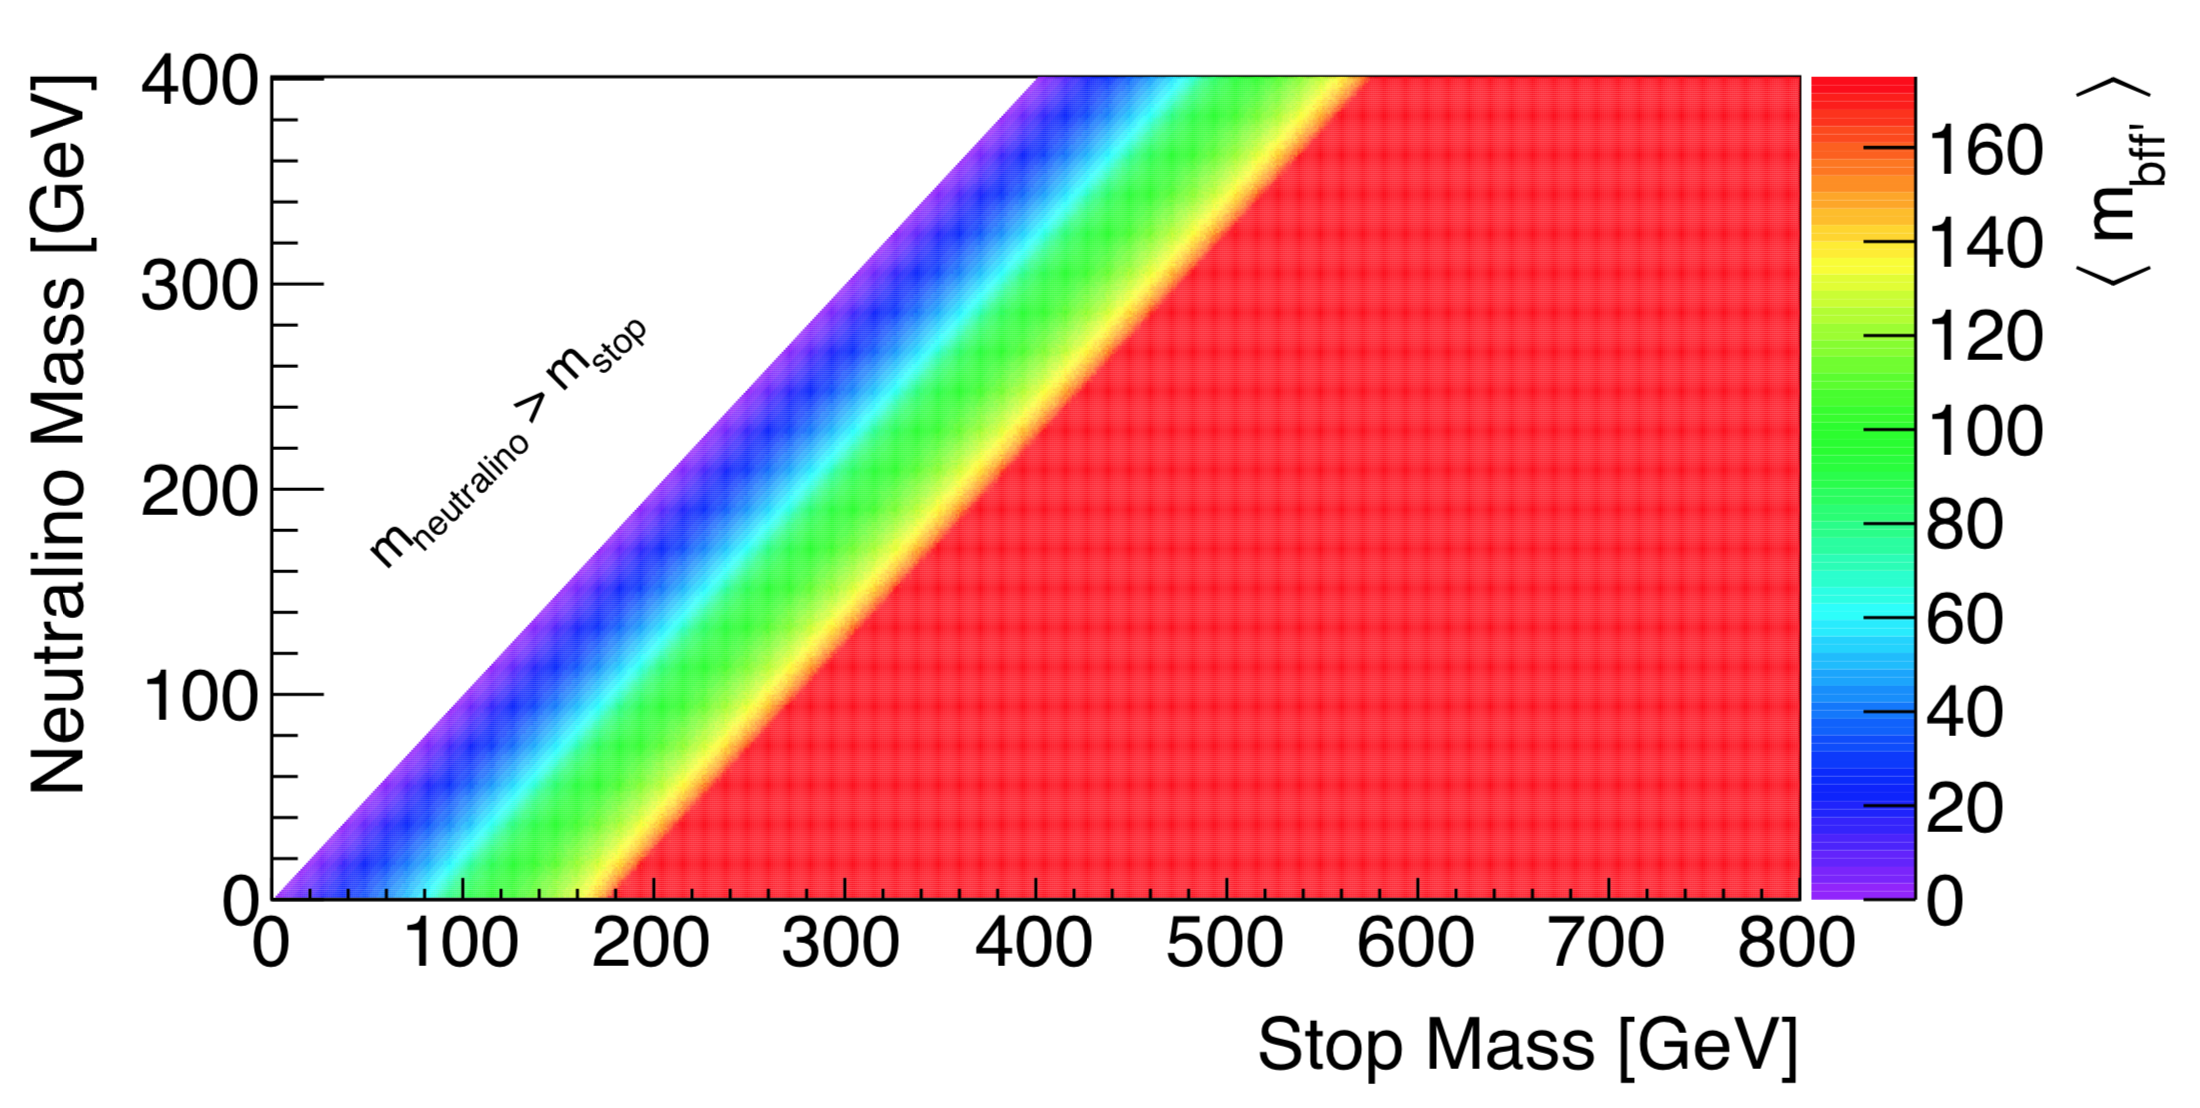
\includegraphics[width=0.75\textwidth]{figures/search_stop2l/nachman_stop_phase_space}
        \caption{
            Average invariant mass of the $b$-quark and SM fermions ($f f^{\prime}$) in the
            final state of the $\stopone \rightarrow b f f^{\prime} \ninoone$ decay, as a function of the mass
            of the \stopone and \ninoone particles.
            Figure taken from Ref.~\cite{Nachman:2016qyc}.
        }
        \label{fig:stop_phase_space}
    \end{center}
\end{figure}

% near the boundaries, blah blah blah it is important to get the simulation
% of the spin etc correct ---> MADSPIN

% the effects of stop mixing are particularly exageratted in the regions
% near ∆M = m_top, and so MadSpin...
% these effects are in addition to the kinematic considerations described in the itemized list in the previous section...
% --> THAT IS: PHASE SPACE AND POLARIZATION INFO ACCEPTS THE SIGNAL ACCEPTANCE
%  \cite{Belanger:2012tm,Perelstein:2008zt,Low:2013aza}

\subsection{Aside: SUSY Signal Grids}
\label{sec:susy_signal_grid}

Before the search for the \stopone can begin, MC simulated samples representing this process
must be obtained.
Once a given simplified model of the MSSM is chosen, specific points in the
$(m_{\stopone}, m_{\ninoone})$-plane are chosen and for each a separate MC simulated
sample is produced.
Each point represents a different hypothesis of SUSY, characterised by the specific masses
of the \stopone and \ninoone sparticles.
In ATLAS, this process of choosing points in the SUSY parameter space to produce MC simulated samples
is one requiring high levels of deliberation and discussion.
This is due to the fact that the simulation of complicated physics processes requires large amounts
of ATLAS' CPU resources, of which any given analysis group only has so much allocated, and so, among other things,
judicious choices about the number of events to be simulated at each point in the $(m_{\stopone}, m_{\ninoone})$-plane
must be made, as well as careful consideration of previous analyses' exclusion coverage in the same parameter space.
For this reason, the resulting SUSY `signal grids' are \textit{sparse}, as illustrated in Figure~\ref{fig:susy_signal_grid}.
Depending on how sparse the produced signal grid is, how the points are grouped, or how large each MC-sample at each
point is (in terms of number of MC events simulated), the resulting analyses' conclusions
can result in unphysical or even discontinous exclusion regions, which is clearly the case in the Run 1 searches
for the three-body decay of the \stopone, seen in Figure~\ref{fig:run1_stop_summary}.
When interpreting the results of SUSY searches, then, it is important to keep these facts in mind
so as to not over-interpret the results' statements about any fine-grained details of SUSY parameter space to
which the analyses are generally not sensitive.
Each point in a SUSY signal grid allows, rather, an analysis to make general statements about
an \textit{extended}, but still local, region of parameter space under the assumed simplified model.

\begin{figure}[!htb]
    \begin{center}
        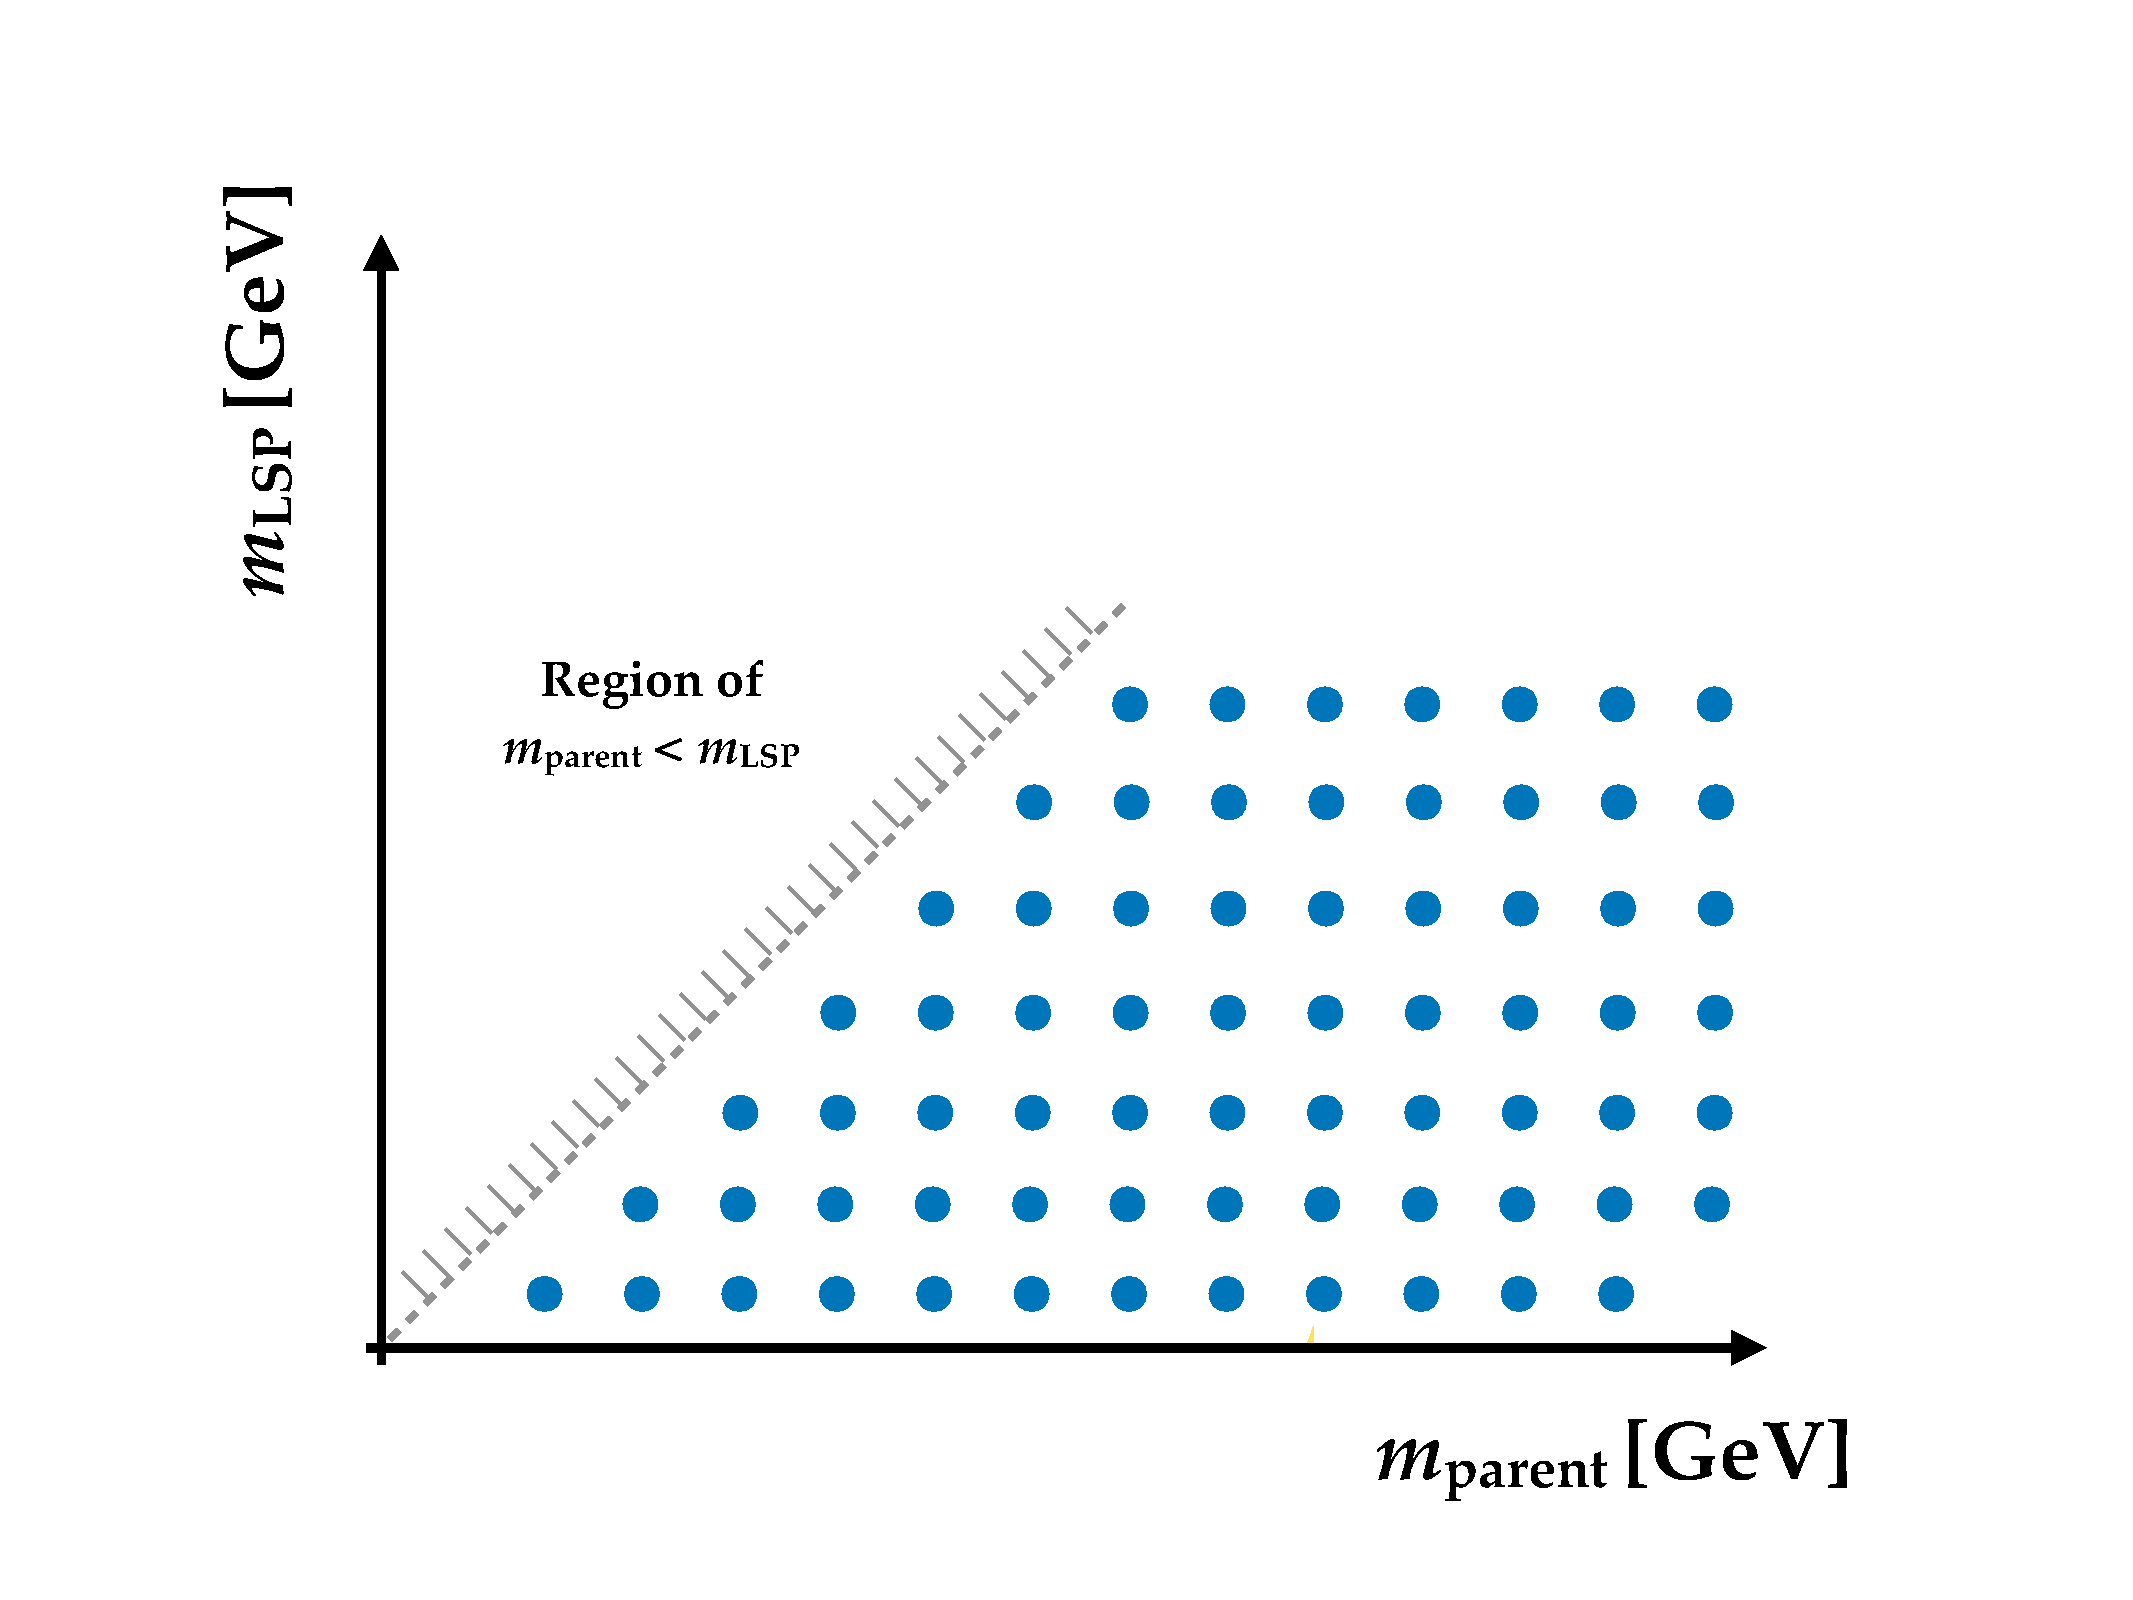
\includegraphics[width=0.6\textwidth]{figures/search_stop2l/signal/susy_signal_grid_example}
        \caption{
            Illustration of a SUSY signal grid.
            The blue points indicate points in the simplified model parameter space for which
            an individual MC-simulated sample is produced and available for use in analyses
            searching for the given type of SUSY.
        }
        \label{fig:susy_signal_grid}
    \end{center}
\end{figure}

\subsection{Simulation of the Three-body Decay of the Stop Quark}
\label{sec:stop_sim}

The MC simulation of the three-body decay of the \stopone, used in the analysis discussed in 
this chapter, is performed using \textsc{MadGraph5\_AMC@NLO}, including diagrams with up to
two additional partons.
In the three-body region of phase space of the \stopone decays, proceeding primarily via off-shell
intermediate SM top-quarks, the preservation of the \stopone left-right polarisation information
must be handled with care.\footnote{The
\stopone is of course a scalar particle, so it not chiral.
The \stopL and \stopR  states that make up the \stopone and \stoptwo mass eignestates refer, instead, 
to their corresponding SM superpartner counterparts.
}
For this reason, produced \stop sparticles provided by \textsc{MadGraph5\_AMC@NLO} are decayed
via \textsc{MadSpin}, described in Section~\ref{sec:mc_gen_afterburner}, which properly
propagates the polarisation information of the massive \stopone particle into the
off-shell and intermediate SM top-quark to which it decays, such that the kinematics of the
$W$-boson ($\ell \nu$ system) and $b$-quark are correct.
\textsc{Pythia} is used for the showering and fragmentation.

\subsection{Description of the Three-body Decay Final State}
\label{sec:stop_final_state}

% figure stop_phase_space, indicates soft decay products from the stop decays:
%  -> soft b-quarks == stop b-jets, not reconstructuble
%  -> soft W-bosons that are still on-shell --> lepton pT/kinematics similar to that of WW production,
%       especially given that the b-jets are missing for large portions of the three-body phase space
%  -> soft \ninoone == generally low values of the missing transverse moemnetum, as compared to the two-body
%       region, again this makes it more like WW production in the region nearer to the ∆M = m_W diagonal.
